\documentclass{jsarticle}
\usepackage{listings,jvlisting} % 日本語のコメントアウトをする場合jvlistingが必要
\usepackage{color} % ソースコードの色塗り
\usepackage[dvipdfmx]{graphicx}
\usepackage{amsmath,amssymb} % 数式
\usepackage{here}

\usepackage[%
 dvipdfmx,% 欧文ではコメントアウトする
 setpagesize=false,%
 bookmarks=true,%
 bookmarksdepth=3,%
 bookmarksnumbered=true,%
 colorlinks=false,%
 pdftitle={},%
 pdfsubject={},%
 pdfauthor={},%
 pdfkeywords={}%
]{hyperref}


\lstset{
  basicstyle={\ttfamily},
  identifierstyle={\small},
  commentstyle={\smallitshape},
  keywordstyle={\small\bfseries},
  ndkeywordstyle={\small},
  stringstyle={\small\ttfamily},
  frame={tb},
  breaklines=true,
  columns=[l]{fullflexible},
  numbers=left,
  xrightmargin=0zw,
  xleftmargin=3zw,
  numberstyle={\scriptsize},
  stepnumber=1,
  numbersep=1zw,
  lineskip=-0.5ex
}

\begin{document}
\title{応用データ解析中間レポート}
\author{03230966 河田顕帆}
\maketitle

本レポート作成に用いたソースコードは\href{https://github.com/takeshiho0531/UTokyo-assignment/blob/bf90c0d5bb43624e2a78c65f54a0b9647537abd1/3A/applied_data_analysis/mid_report/%E5%BF%9C%E7%94%A8%E3%83%87%E3%83%BC%E3%82%BF%E8%A7%A3%E6%9E%90%E8%AA%B2%E9%A1%8C%E4%B8%AD%E9%96%93%E8%AA%B2%E9%A1%8C.ipynb}{github}にて公開している。\\

\section{課題1}
期待値・中央値・標本分散・不偏分散・歪度・尖度は以下のようにして計算した。\\

\begin{lstlisting}
import numpy as np
import pandas as pd

df = pd.read_csv('BostonHousing.csv')

medv_data = df['MEDV']

# 期待値(平均値)
mean_medv = np.mean (medv_data)

# 中央値
median_medv = np.median (medv_data)

# 標本分散
sample_variance_medv = np.var (medv_data, ddof=0)

# 不偏分散
unbiased_variance_medv = np.var (medv_data, ddof=1)

# 歪度
skewness_medv = medv_data.skew ()

# 尖度
kurtosis_medv = medv_data.kurtosis ()

\end{lstlisting}

結果は以下のようになった。
\begin{itemize}
  \item 期待値(平均値): 22.532806324110677
  \item 中央値: 21.2
  \item 標本分散: 84.41955615616556
  \item 不偏分散: 84.58672359409856
  \item 歪度: 1.1080984082549072
  \item 尖度: 1.495196944165818
\end{itemize}

平均値よりも中央値の方が小さい値を取っているため、データは左に歪んでいると言える。歪度に関しては、正の歪度があることを示しており、データは右裾が長いと言える。
尖度に関しては1.5となっているため、尖度が0の正規分布よりも尖っていて、正規分布よりも価格のピークが集中していることが分かる。
実際にヒストグラムを描画してみると、以下のようになり、上記の事柄が確かめられる。\\
\begin{figure}[H]
  \centering
  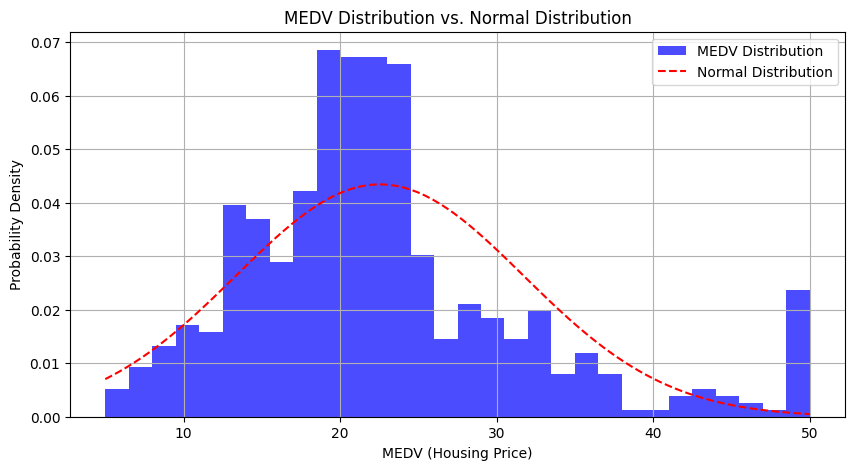
\includegraphics[width=15cm]{histogram.png}
\end{figure}

\section{課題2}
データ内の各変数の共分散行列をheatmapにして図示すると以下のようになる。 \\
MEDVと相関係数の絶対値が比較的大きい変数はLSTAT (相関係数:-0.74)とRM (相関係数:0.70)であることが分かる。
逆に、相関係数の絶対値が比較的小さい変数はCHAS (相関係数:0.18)とDIS (相関係数:0.25)であることが分かる。\\
\begin{figure}[H]
  \centering
  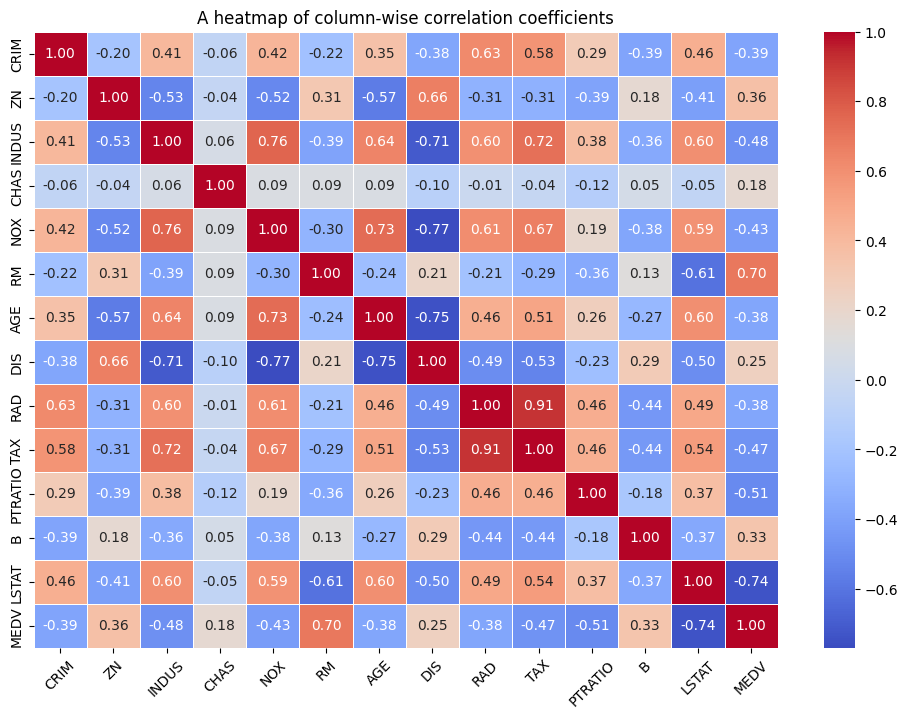
\includegraphics[width=15cm]{heatmap.png}
\end{figure}

\begin{itemize}
  \item 相関係数の絶対値が大きい変数
    \begin{itemize}
      \item LSTAT \\
      人口の低所得者の割合と価格の負の相関がある。これは、低所得者の割合が高い地域ほど価格が安いということを示している。
      \item RM \\
      1戸あたりの平均部屋数と価格の正の相関がある。これは、部屋数が多いほど価格が高いということを示している。
    \end{itemize}
  \item 相関係数の絶対値が小さい変数
    \begin{itemize}
      \item CHAS \\
      チャールズ川沿いかどうかと価格の相関が小さい。これは、チャールズ川沿いかどうかと価格にはあまり関係がないということを示している。
      \item DIS \\
      ボストンの主な雇用センターまでの重み付き距離と価格の相関が小さい。これは、雇用センターまでの距離と価格にはあまり関係がないということを示している。
    \end{itemize}
\end{itemize}


\end{document}